\quad{}
\item \textbf{{[}ALVL/9597/2013/P1/Q3{]} }

The task is to store a dataset (maximum size 20 items) as a binary
tree structure. You should assume that the data items are unique.

The program will use a user-defined type Node for each node defined
as follows:
\begin{center}
\begin{tabular}{|l|l|l|}
\hline 
\texttt{\hspace{0.01\columnwidth}}Identifier & \texttt{\hspace{0.01\columnwidth}}Data Type & \texttt{\hspace{0.05\columnwidth}}Description\tabularnewline
\hline 
\texttt{LeftP} & \texttt{INTEGER} & The left pointer for the node\tabularnewline
\hline 
\texttt{Data} & \texttt{STRING} & The node's data value\tabularnewline
\hline 
\texttt{RightP} & \texttt{INTEGER } & The right pointer for the node\tabularnewline
\hline 
\end{tabular}
\par\end{center}

A linked list is maintained of all the unused nodes which do not form
part of the tree. The first available node which is used for a new
term is indicated by NextFreePosition. Items in the unused list are
linked using their left pointers.

The binary tree and linked list are implemented using variables as
follows:
\begin{center}
\begin{tabular}{|l|l|l|}
\hline 
\texttt{\hspace{0.01\columnwidth}}Identifier & \texttt{\hspace{0.01\columnwidth}}Data Type & \texttt{\hspace{0.05\columnwidth}}Description\tabularnewline
\hline 
\texttt{ThisTree} & \texttt{ARRAY{[}20{]} : Node} & The tree data\tabularnewline
\hline 
\texttt{Root } & \texttt{INTEGER} & Index for the root position of the \texttt{ThisTree} array\tabularnewline
\hline 
\texttt{NextFreePosition} & \texttt{INTEGER } & Index for the next unused node\tabularnewline
\hline 
\end{tabular}
\par\end{center}

\begin{center}
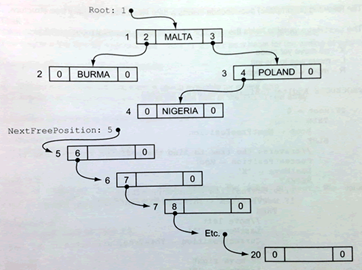
\includegraphics[width=0.5\paperwidth]{C:/Users/Admin/Desktop/Github/question_bank/LyX/static/img/9597-ALVL-2013-P1-Q3}
\par\end{center}

The diagram shows the binary tree and linked list after four values
have been added.

\subsubsection*{Task 3.1}

Write the program code to declare all the required variables and create
the initial linked list which contains all 20 nodes. Add statement(s)
to initialise the empty tree.

\hfill{}{[}10{]}

\subsubsection*{Evidence 7}

Your program code for Task 3.1. {[}11{]}

The following (incomplete) pseudocode inserts a data value into the
binary tree structure.

The \texttt{LastMove} variable holds the direction of the previous
traversal move as follows:

X - no move yet made 

L - move was to the left 

R - move was to the right

\noindent %
\noindent\begin{minipage}[t]{1\columnwidth}%
\texttt{PROCEDURE AddItemToBinaryTree(NewFreeItem)}

\texttt{\qquad{}IF Root = 0}

\texttt{\qquad{}\qquad{}THEN}

\texttt{\qquad{}\qquad{}\qquad{}Root \textleftarrow{} NextFreePosition}

\texttt{\qquad{}\qquad{}ELSE}

\texttt{\qquad{}\qquad{}\qquad{}// traverse the tree to find the
position for the new value}

\texttt{\qquad{}\qquad{}\qquad{}CurrentPosition \textleftarrow{}
Root}

\texttt{\qquad{}\qquad{}\qquad{}LastMove \textleftarrow{} 'X'}

\texttt{\qquad{}\qquad{}\qquad{}REPEAT}

\texttt{\qquad{}\qquad{}\qquad{}\qquad{}PreviousPosition \textleftarrow{}
CurrentPosition}

\texttt{\qquad{}\qquad{}\qquad{}\qquad{}IF NewFreeItem < ThisTree{[}CurrentPosition{]}.Data}

\texttt{\qquad{}\qquad{}\qquad{}\qquad{}\qquad{}THEN}

\texttt{\qquad{}\qquad{}\qquad{}\qquad{}\qquad{}\qquad{}// move
left}

\texttt{\qquad{}\qquad{}\qquad{}\qquad{}\qquad{}\qquad{}LastMove
\textleftarrow{} 'L'}

\texttt{\qquad{}\qquad{}\qquad{}\qquad{}\qquad{}\qquad{}CurrentPosition
\textleftarrow{} ThisTree{[}CurrentPosition{]}.LeftP}

\texttt{\qquad{}\qquad{}\qquad{}\qquad{}\qquad{}ELSE}

\texttt{\qquad{}\qquad{}\qquad{}\qquad{}\qquad{}\qquad{}// move
right}

\texttt{\qquad{}\qquad{}\qquad{}\qquad{}\qquad{}\qquad{}LastMove
\textleftarrow{} 'R'}

\texttt{\qquad{}\qquad{}\qquad{}\qquad{}\qquad{}\qquad{}CurrentPosition
\textleftarrow{} ThisTree{[}CurrentPosition{]}.RightP}

\texttt{\qquad{}\qquad{}\qquad{}\qquad{}ENDIF}

\texttt{\qquad{}\qquad{}\qquad{}UNTIL CurrentPosition = 0}

\texttt{\qquad{}ENDIF}

\texttt{\qquad{}IF LastMove = 'R'}

\texttt{\qquad{}\qquad{}THEN}

\texttt{\qquad{}\qquad{}\qquad{}ThisTree{[}PreviousPosition{]}.RightP
\textleftarrow{} NextFreePosition}

\texttt{\qquad{}\qquad{}ELSE}

\texttt{\qquad{}\qquad{}\qquad{}ThisTree{[}PreviousPosition{]}.LeftP
\textleftarrow{} NextFreePosition}

\texttt{\qquad{}ENDIF}

\texttt{\qquad{}NextFreePosition ThisTree{[}NextFreePosition{]}.LeftP}

\texttt{ENDPROCEDURE}%
\end{minipage}

Note: The above text is available in the text file \texttt{PSEUDOCODE\_TASK\_3\_2.TXT}

\subsubsection*{Task 3.2}

Write non-recursive code to implement the \texttt{AddItemToBinaryTree}
procedure. You may use the text file \texttt{PSEUDOCODE\_TASK\_3\_2.TXT}
as a basis for the writing of your code.

The given pseudocode is incomplete as:
\begin{itemize}
\item it does not initially test that there is space available for a new
item 
\item it does not assign \texttt{NewTreeItem} to the data field of the \texttt{ThisTree}
array
\end{itemize}
Add these requirements to your program solution.

\subsubsection*{Evidence 8}

Your program code for Task 3.2.\hfill{} {[}6{]}

\subsubsection*{Task 3.3}

Write a procedure\texttt{ OutputData} which displays the value of
\texttt{Root}, the value of \texttt{NextFreePosition} and the contents
of \texttt{ThisTree} in index order.

\subsubsection*{Evidence 9}

Your program code for Task 3.3. \hfill{}{[}5{]}

\subsubsection*{Task 3.4}

Write a main program to:
\begin{itemize}
\item Input new data items and add them to the binary tree by calling procedure
\texttt{AddItemToBinaryTree}. The input is terminated with value \textquotedbl\texttt{XXX}\textquotedbl .
Do not attempt to validate the input of the country names. 
\item Your program will then call procedure \texttt{OutputData}.
\end{itemize}
Run the program with the input of the single value \textquotedbl\texttt{XXX}\textquotedbl .

\subsubsection*{Evidence 10}

Screenshot showing the output from running the program in Task 3.4.\hfill{}
{[}3{]}

\subsubsection*{Task 3.5}

Test your program using the following data items input in the order
shown:
\begin{center}
\texttt{INDIA, NEPAL, MALAYSIA, SINGAPORE, BURMA, CANADA, LATVIA,
XXX}
\par\end{center}

\subsubsection*{Evidence 11}

Provide screenshot test evidence for Task 3.5. \hfill{}{[}5{]}

Further program code is required to carry out an \textbf{in-order
traversal}.

\subsubsection*{Task 3.6}

Write a recursive procedure to carry out an in-order tree traversal. 

Include a call to the procedure from your main program.

\subsubsection*{Evidence 12}

Your program code. \hfill{}{[}8{]}

\subsubsection*{Evidence 13}

Produce a screenshot for the Task 3.5 dataset confirming the output
of the countries in alphabetical order. \hfill{}{[}2{]}